% !TeX spellcheck = de_DE
\documentclass{uebung_cs}
\usepackage{algo221}
\uebung{5}{}{}
\blattname{Übungen zu Woche 5: Randomisierte Algorithmen I}

%%%%%%%%%%%%%%%%%%%%%%%%%%%%%%%%%%%%%%%%%%%%%%%%%%%%%%%%%%%%%%%%%%%%%%%%%%%%
\begin{document}

Das Übungsblatt enthält alle empfohlenen Lernaktivitäten für die aktuelle Woche.

\begin{itemize}
\item \textbf{Heimarbeit bis Montag 17:00.}
    \begin{itemize}
    \item 
    Schau die Videos an und lies die Buchkapitel.
    \item Bearbeite die \emoji{seedling}-Aufgabe in \href{https://moodle.studiumdigitale.uni-frankfurt.de/moodle/course/view.php?id=2241}{Moodle}. (Feste Abgabefrist!)
    \item Lese den Aufgabentext aller Übungsaufgaben.
    \end{itemize}
\item \textbf{Heimarbeit.} Bearbeite die Übungsaufgaben soweit möglich. Probier zumindest alle mal!
\item \textbf{Dienstag/Donnerstag.}
\begin{itemize}
    \item \textbf{8:00--8:15.} Besprechung im Hörsaal.
    \item \textbf{8:15--9:15.} Bearbeite jetzt die Übungen, die du noch nicht lösen konntest. Sprich mit anderen Studis! Frag das Vorlesungsteam um Hilfe!
    \item \textbf{9:15--9:45.} Lösungsspaziergang zu den Aufgaben für heute.
\end{itemize}

\item \textbf{Heimarbeit bis Freitag, den 19.11., 17:00.} Gib deine Lösungen zu der \emoji{star}-Aufgabe von diesem Übungsblatt in \href{https://moodle.studiumdigitale.uni-frankfurt.de/moodle/course/view.php?id=2241}{Moodle} ab. (Feste Abgabefrist!)
\end{itemize}

\section*{Dienstag}

\begin{exercise}[Wahrscheinlichkeitsrechnung]\
	% Algorithms and Data Structures 2 - randomizedI.pdf
	\begin{enumerate}
		\item 
		Seien $E$ und $F$ zwei Ereignisse, für die $\Pr(E | F) = \Pr(E)$ und $\Pr(F | E) = P(F)$ gelten. Zeige, dass dann auch $\Pr(E \cap F) = \Pr(E) \cdot \Pr(F)$ gilt.
		\item Betrachte \textit{contention resolution} mit $n$ Prozessen. Betrachte die folgende Anwendung der \textit{union bound} aus der Vorlesung:
		\[
			\Pr\left(\bigcup_{i=1}^n F_{i,t}\right)
			\le
			\sum_{i=1}^n \Pr(F_{i,t})\,.
		\]
		Hierbei ist $F_{i,t}$ das Ereignis, dass Prozess $i$ es in keiner der Runden $1,\dots,t$ geschafft hat, auf die Datenbank zuzugreifen.
		Sind die einzelnen Ereignisse~$F_{i,t}$ hierbei disjunkt oder überschneiden sie sich?
	\end{enumerate}
\end{exercise}

\begin{exercise}[Contention Resolution]\
	% Algorithms and Data Structures 2 - randomizedI.pdf
	Führe das \textit{contention resolution} Protokoll mit $4$ Prozessen von Hand aus. Benutze hierzu zwei Münzen und werfe sie, um die zufällige Auswahl zu simulieren.
	Wie viele Runden hast du gebraucht, bis alle Prozesse erfolgreich auf die Datenbank zugegriffen haben?
	Inwiefern passt dein Ergebnis zu der theoretisch vorhergesagten Anzahl an benötigten Runden zusammen?
\end{exercise}    

\begin{exercise}[Minimaler Schnitt]
	% Algorithms and Data Structures 2 - randomizedI.pdf
	Betrachte den Beispielgraphen zum Kontraktionsalgorithmus aus der Vorlesung:
	\begin{center}
	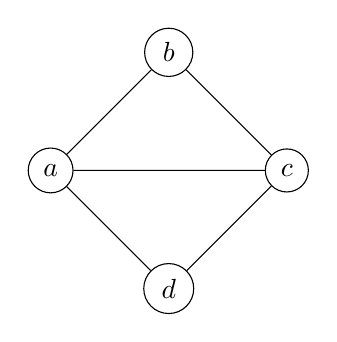
\begin{tikzpicture}
            \node[draw,circle] (a) at (0,0) {$a$};
            \node[draw,circle] (b) at (1.5,1.5) {$b$};
            \node[draw,circle] (d) at (1.5,-1.5) {$d$};
            \node[draw,circle] (c) at (3,0) {$c$};
            
            \draw  (a) -- (b)
                   (a) -- (c)
                   (a) -- (d)
                   (b) -- (c)
                   (c) -- (d);
        \end{tikzpicture}
	\end{center}
	\begin{enumerate}
		\item Zeige, dass es eine Sequenz von Kontraktionen gibt, die zu einem nicht minimalen Schnitt führt.
		\item Berechne die genaue Wahrscheinlichkeit, dass der Kontraktionsalgorithmus den minimalen Schnitt ausgibt.
	\end{enumerate}
\end{exercise}

\section*{Donnerstag}

\begin{exercise}[Schneller Kontraktionsalgorithmus]
	% Algorithms and Data Structures 2 - randomizedI.pdf
	Wie kann man den Kontraktionsalgorithmus für minimale Schnitte effizient implementieren? Beschreibe alle nötigen Datenstrukturen und Algorithmen und analysiere die Laufzeit sowie den Platzverbrauch.
\end{exercise}

\begin{exercise}[Kontraktionsalgorithmus analysieren]
	% Algorithms and Data Structures 2 - randomizedI.pdf
	Betrachte die folgende Analyse der Erfolgswahrscheinlichkeit für den Kontraktionsalgorithmus. Die folgende Herleitung führt zum gewünschten Ergebnis:
	\begin{align}
		&\nonumber\Pr(E_{n-2} \cap \cdots \cap E_1) \\
		&= \Pr(E_{n-3} \cap \cdots \cap E_1) \cdot \Pr(E_{n-2}|E_{n-3} \cap \cdots \cap E_1) \\
		&= \Pr(E_1) \cdot \Pr(E_2|E_1) \cdots \Pr(E_{j+1} | E_j \cap \cdots \cap E_1) \cdots \Pr(E_{n-2} | E_{n-3} \cap \cdots \cap E_1) \\
		&\ge \left(1 - \frac{2}{n} \right) \cdot \left(1 - \frac{2}{n-1} \right) \cdot \left(1 - \frac{2}{n-2} \right) \cdots \left(1 - \frac{2}{3} \right) \\
		&= \left(\frac{n-2}{n}\right) \cdot \left(\frac{n-3}{n-1}\right) \cdot \left(\frac{n-4}{n-2}\right) \cdots \left(\frac{2}{4}\right) \cdot \left(\frac{1}{3}\right) \\
		&= \left(\frac{2}{n(n-1)}\right) \geq \frac{2}{n^2}
	\end{align}
	\begin{enumerate}
		\item Benutze zwei verschiedene Wege, um (1) zu zeigen. Erstens, indem du die Formel für die bedingte Wahrscheinlichkeit benutzt. Zweitens, mache dir bewusst, was die linke und rechte Seite bedeuten.
		\item Zeige (2). 
		\item[] \textit{Hinweis:} Benutze das Ergebnis aus Teilaufgabe a)
		\item Schätze jeden Faktor einzeln ab, um (3) zu zeigen. 
		\item Zeige (4).
		\item Zeige (5).
	\end{enumerate}
\end{exercise}

\begin{exercise}[Mehrheit]
	% Algorithms and Data Structures 2 - randomizedI.pdf
	Gegeben ist eine Sequenz $x_1,x_2,\dots,x_n$ von $n$ ganzen Zahlen. Die Sequenz hat das \textit{Mehrheitselement}~$t$, wenn die Zahl $t$ öfter als $\frac{n}{2}$-mal in der Sequenz vorkommt. Zum Beispiel hat die Sequenz $1,2,3,1,2,2,2$ das Mehrheitselement $2$, während die Sequenz $2,2,1,2,3,3$ kein Mehrheitselement hat. Im Folgenden ist der randomisierter Algorithmus \textsc{FindeMehrheitsElement} beschrieben, der das Mehrheitselement finden soll.
	
	\begin{quote}
		\textsc{FindeMehrheitsElement}: \\
		Ziehe eine uniform zufällige Zahl $x_i$ aus der Sequenz. Prüfe dann, ob $x_i$ öfter als $\frac{n}{2}$-mal in der Sequenz vorkommt. Wenn ja, dann ist $x_i$ das Mehrheitselement. Wenn das nicht der Fall ist, gibt der Algorithmus aus, dass es kein Mehrheitselement gibt.
	\end{quote}
	\begin{enumerate}
		\item Was ist die Laufzeit von \textsc{FindeMehrheitsElement}?
		\item Kann \textsc{FindeMehrheitsElement} ein Mehrheitselement zurückgeben, wenn die Sequenz keines hat? Begründe deine Antwort.
		\item Kann \textsc{FindeMehrheitsElement} ausgeben, dass kein Mehrheitselement existiert, obwohl die Sequenz ein solches besitzt? Begründe deine Antwort.
		\item Bestimme die Wahrscheinlichkeit, dass \textsc{FindeMehrheitsElement} eine falsche Antwort liefert.
	\end{enumerate}
\end{exercise}

\newpage
\section*{Sternaufgabe}

\begin{exercise}[\emoji{star}: Zufällige Konfliktfreiheit]
	In Abschnitt 13.1 (\textbf{KT}) haben wir ein einfaches verteiltes Protokoll gesehen, um ein \textit{contention resolution} Problem zu lösen. Eine zweite Möglichkeit, um \textit{contention resolution} mittels Randomisierung zu lösen, ist eine verteilte Konstruktion eines Independent Set.

	In einem System mit $n$ Aufgaben stehen einige Paare von Aufgaben miteinander im Konflikt, beispielsweise wenn beide Aufgaben Zugang zu derselben Ressource brauchen. Das Ziel ist es, in einem gegebenen Zeitintervall eine möglichst große Menge~$S$ von ausführbaren Aufgaben zu finden, sodass keine zwei Aufgaben aus $S$ in einem Konflikt stehen. Die Menge~$S$ nennen wir \textit{konfliktfrei}.
	
	Diesen Vorgang kann man sich als einen Graphen $G = (V,E)$ vorstellen. Dabei repräsentiert jeder Knoten $v \in V$ eine Aufgabe und eine Kante $e = (u,v)$ stellt einen Konflikt zwischen zwei Aufgaben $u$ und $v$ dar. Ist eine Menge~$S$ von Aufgaben konfliktfrei, bilden sie eine \emph{unabhängige Menge} (\emph{independent set}) in $G$. 
	Da man das allgemeine Independent Set Problem auf dieses Problem reduzieren kann, ist es schwierig, eine maximale und konfliktfreie Menge $S$ für einen beliebigen Konfliktgraphen $G$ zu finden. 
	
	Deshalb benutzen wir eine Heuristik mit einer einfachen dezentralisierten Methode, die eine vernünftig große und konfliktfreie Menge findet: Jede Aufgabe kommuniziert nur mit einer kleinen Anzahl anderer Aufgaben und entscheidet dann, ob sie in die Menge~$S$ gehört oder nicht.
	Wir nehmen an, dass jeder Knoten genau $d$ Nachbarn in $G$ hat. Das heißt, jede Aufgabe hat einen Konflikt zu genau $d$ anderen Aufgaben. Schaue dir nun das folgende Verfahren an:
	
	\begin{quote}
		\textsc{FindeKonfliktfreieMenge}: \\
		Jede Aufgabe $P_i$ wählt unabhängig einen zufälligen Wert $x_i$. Dabei nimmt $x_i$ mit einer Wahrscheinlichkeit von $\frac{1}{2}$ den Wert $0$ und mit einer Wahrscheinlichkeit von $\frac{1}{2}$ den Wert $1$ an. Die Aufgabe kommt genau dann in die Menge $S$, wenn sie $x_i = 1$ gewählt hat und jede Aufgabe, mit der sie im Konflikt steht, den Wert $0$ gewählt hat.
	\end{quote}
	
		\begin{enumerate}
		\item Beweise, dass die durch \textsc{FindeKonfliktfreieMenge} entstehende Menge~$S$ immer konfliktfrei ist.
		\item Gib außerdem eine Formel für die erwartete Größe von $S$ in Abhängigkeit der Anzahl $n$ an Aufgaben und der Anzahl~$d$ an Konflikten pro Aufgabe an. Begründe, warum deine Formel korrekt ist.
	\end{enumerate}
\end{exercise}

\end{document}
